\section{Ανάπτυξη Αθροιστών υπολοίπου $2^n-1$ }

Σε αυτό το κεφάλαιο θα αναπτυχθούν συνολικά δώδεκα αθροιστές υπολοίπου $2^n-1$
ακολουθώντας την αρχιτεκτονική που παρουσιάστηκε στο προηγούμενο κεφάλαιο 
με τα ελάχιστα επίπεδα. Ανάλογα με το είδος της παραγοντοποίησης που τους εφαρμόζεται 
οι αθροιστές ομαδοποιούνται σε τρεις ομάδες, Prefix, Ling και Jackson,
και σε κάθε ομάδα θα αναπτυχθεί ένας 8-bit, ένας 16-bit, ένας 32-bit και ένας 64-bit 
αθροιστής. Κάθε αθροιστής που αναπτύσσεται περιγράφεται πλήρως από τις λογικές 
συναρτήσεις κάθε επιπέδου του.

Για την περιγραφή των κυκλωμάτων χρησιμοποιήθηκε η γλώσσα περιγραφής υλικού Verilog \cite{1620780}, ενώ η προσομοίωση και ο έλεγχος ορθής περιγραφής και λειτουργίας υλοποιείται
με την χρήση του εργαλείου VCS της Synopsys \cite{vcs-synopsys}. Επίσης, για την καλύτερη
βελτιστοποίηση επιλέχθηκε η περιγραφή των κυκλωμάτων να γινεί σε αρκετά χαμηλό επίπεδο. Κάθε
κόμβος που αντιπροσωπεύει μια λογική συνάρτηση περιγράφηκε σε ξεχωριστή μονάδα. Όμως στις 
περιπτώσεις όπου η είσοδος των αθροιστών είναι μεγάλη θα έπρεπε να γίνουν αρκετές κλήσεις των 
verilog-modules στον κώδικα. Για παράδειγμα, με μήκος εισόδου 64 δυαδικά ψηφία, μόνο και μόνο οι 
μονάδες που υπολογίζουν τα σήματα generate και propagate καλούνται 64 φορές και δεν
έχει ακόμα αρχίσει η περιγραφή του δέντρου, πράγμα που καθιστά την γραφή του κώδικα 
δύσκολη. Για την αποφυγή ανθρώπινων λαθών, τα οποία θα καθυστερούσαν πολύ την 
διαδικασία του ελέγχου, αναπτύχθηκε κώδικας σε python για την εκτύπωση της Verilog
περιγραφής του κάθε αθροιστή.




\subsection{Βασική δομή}
Στην ενότητα \ref{section:jackson} έγινε μια αναφορά σε σχεδιαστικούς κανόνες όσο αφορά τους 
αθροιστές Jackson. Για την ανάπτυξη ενός Jacson αθροιστή υπάρχει ένα μεγάλο πλήθος πιθανών υλοποιήσεων,
όχι μόνο στην επιλογή του προθεματικού δέντρου και το πλήθος των όρων της παραγοντοποίησης ( Radix-2, 
Radix-3, Radix-4 ... ), κάτι που αφορά και τους αθροιστές Prefix και Ling, αλλά 
και στην επιλογή της συνάρτησης παραγοντοποίησης σε κάθε επίπεδο.
% \\
% \textcolor{red}{[Γράψε όλους τους συνδυασμούς για έναν 8-bit ή 16-bit αθροιστή σε συντομία
% π.χ. για 8 = 2x2x2, 2x4, 4x2 , και σε κάθε ένα τις πιθανές Burgess Συναρτήσεις]}\\

Όσο αφορά την επιλογή του πλήθους εισόδων στους κόμβους του κάθε επίπεδου αποφεύγεται
η επιλογή του Radix-2 διότι, επαναδιατυπώνοντας, οι συναρτήσεις κατά Jacskon δεν διαφέρουν 
με αυτές ενός απλού Prefix. Θα ήταν αρκετά αποδοτική η υλοποίηση ορισμένων επιπέδων με Radix-3
, όπως και στους αθροιστές που αναπτύχθηκαν στα \cite{6189978} και \cite{6810474}, διότι
στις περιπτώσεις περισσότερων των δύο εισόδων έχει εφαρμογή η παραγοντοποίηση και επιπλέον, εφόσον 
οι κόμβοι θα είναι των τριών εισόδων, αρά και οι συναρτήσεις πιο απλές, θα υπάρχουν μεγαλύτερες 
αντιστοιχίες των υλοποιημένων λογικών συναρτήσεων από τις CMOS βιβλιοθήκες. Στην περίπτωση των 
αθροιστών $2^n-1$, με $n=8, 16, 32$ και 64, δεν υπάρχει πολλαπλάσιο του τρία που δίνει τουλάχιστον έναν 
από αυτούς τους αριθμούς. Στην πραγματικότητα υπάρχει τρόπος αλλά το prefix-tree θα διαφέρει αρκετά με αυτό
του Kogge-stone και δεν θα υπάρχει το προνόμιο επαναχρησιμοποίησης κόμβων, με αποτέλεσμα η πολυπλοκότητα των
αθροιστών καθώς η επιφάνεια και κατανάλωση να είναι αρκετά μεγαλύτερες.
Σύμφωνα με αυτά που προειπώθηκαν στον πίνακα \ref{tb:arch_2^n-1} παρουσιάζονται οι επιλογές που έγιναν, οι οποίες
είναι κοινές για κάθε είδος αθροιστή ώστε τα αποτελέσματα των μετρήσεων να είναι έγκυρα.
\begin{table}[H]
\centering
     \begin{tabular}{ || c | c || } 
     \hline
     Μήκος εισόδου & Αρχιτεκτονική\\
     \hline\hline
     8-bit  & 2x4 \\
     16-bit & 4x4 \\
     32-bit & 2x4x4 \\
     64-bit & 4x4x4 \\
     \hline
     \end{tabular}
     \caption{Αρχιτεκτονική δομή των αθροιστών $2^n-1$ προς υλοποίηση}
     \label{tb:arch_2^n-1}
\end{table}

Στην εικόνα \ref{2^8-1_Tree_2x4} παρουσιάζεται προσεγγιστικά η δομή των αθροιστών υπολοίπου $2^8-1$ 
που θα χρησιμοποιηθεί παρακάτω. Ενώ η δομή είναι κοινή και για τα τρία είδη αθροιστών το κάθε σχήμα 
αντιπροσωπεύει διαφορετική λογική συνάρτηση. Επίσης στο δέντρο αυτό ακολουθείται η κατασκευή μόνο 
των σημάτων που οδηγούν τον τελευταίο πολυπλέκτη, δηλαδή στην περίπτωση του Prefix το σήμα G, στου Ling
το σήμα H και στο Jackson το R.
\begin{figure}[H]
\centering
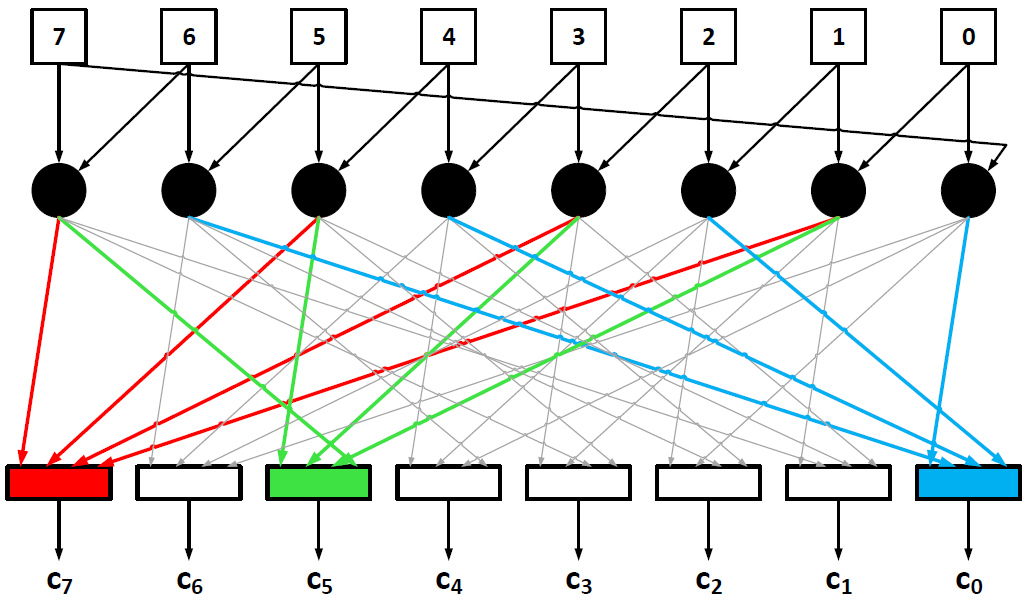
\includegraphics[width=\textwidth]{J8_Color.png}
\caption{Jackson 8-bit $2^n-1$ Adder}
\label{2^8-1_Tree_2x4}
\end{figure}


















\subsection{Διαδικασία ελέγχου ορθής λειτουργίας}
Για τον έλεγχο ορθής λειτουργίας των αθροιστών που αναπτύχθηκαν κατασκευάστηκε ένας αθροιστής 
υπολοίπου $2^n-1$ με την απλούστερη αρχιτεκτονική. Επίσης υλοποιήθηκε μια διαδικασία ελέγχου,
η οποία τροφοδοτεί παράλληλα όλους τους αθροιστές με τυχαίους δυαδικούς αριθμούς και συγκρίνει 
την έξοδο τους με αυτήν των αθροιστών απλής δομής. Αυτός ο έλεγχος επαναλαμβάνεται αρκετές 
φορές, στην περίπτωση αυτή πραγματοποιήθηκαν 10000 επαναλήψεις, με τυχαίο σύνολο αριθμών 
κάθε φορά, για ισχυρότερη πιστοποίηση της ισχυριζόμενης λειτουργίας.
\begin{figure}[H]
\centering
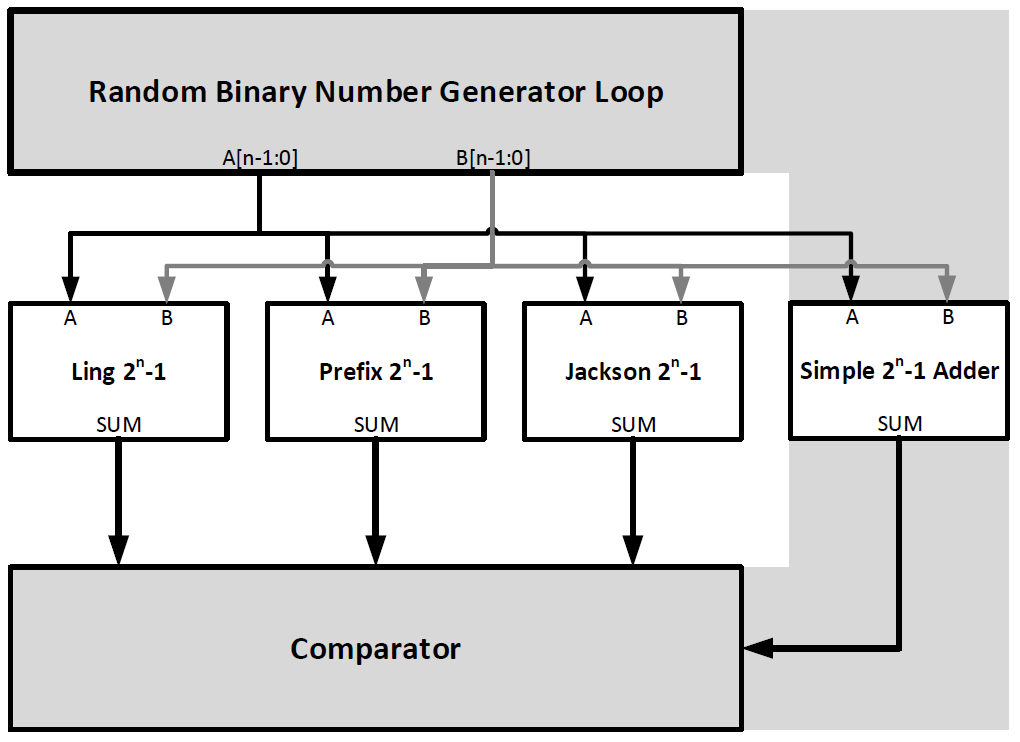
\includegraphics[width=\textwidth]{testbench.png}
\caption{Test-Bench}
\label{fig:testbench}
\end{figure}
Στην εικόνα \ref{fig:testbench} παρουσιάζεται η αρχιτεκτονική του συστήματος ελέγχου. Στην 
μονάδα σύγκρισης ( Comparator ) υπάρχει ένας δείκτης PASS αρχικοποιημένος με την τιμή μηδέν.
Σε κάθε επανάληψη αυξάνεται κατά μία μονάδα αν τα αποτελέσματα προς σύγκριση είναι ίδια.
Στο τέλος των επαναλήψεων το ποσοστό επιτυχίας είναι ίσο με 
\begin{equation*}
    SUCCESS = \frac{PASS}{\text{Number of Test-cycles}}
\end{equation*}
Όπως και σε κάθε περίπτωση σχεδιασμού υλικού πρέπει ο έλεγχος σε επίπεδο προσομοίωσης να
έχει πλήρη επιτυχία, έτσι και σε αυτήν την περίπτωση ένας αθροιστής λειτουργεί σωστά όταν 
στο 100\% των πιθανών διανυσμάτων εισόδου η έξοδος είναι αναμενόμενη σύμφωνα με τον σχεδιασμό.









\subsection{Αλγεβρική περιγραφή των αθροιστών}
\subsubsection{Prefix $2^n-1$}

% -----------------------------------------------------------------------------
% 8-bit
% -----------------------------------------------------------------------------
\begin{table}[H]
\centering
     \begin{tabularx}{\textwidth}{ || c | X || } 

        \hline
        level & P-G Equations\\
        \hline
        \hline
 
        0   & 
        \begin{tabular}{@{}c@{}}
        $g_i = a_i * b_i$\\
        $p_i = a_i + b_i$\\
        $x_i = a_i \oplus b_i $
        \end{tabular}\\\hline

        1 (x2)  & 
        \begin{tabular}{@{}c@{}}
        $G1_i = g_i + p_ig_{i-1}$\\
        $P1_i = p_i * p_{i-1}$
        \end{tabular}\\\hline

        2 (x4)  & 
        \begin{tabular}{@{}c@{}}
        $G2_i = G1_i + P1_{i}G1_{i-2} + P1_{i}P1_{i-2}G1_{i-4} +$ \\ $P1_{i}P1_{i-2}P1_{i-4}G1_{i-6}$
        \end{tabular}\\\hline

        SUM   & 
        \begin{tabular}{@{}c@{}}
        $ sum_i = G_{i-1} \oplus x_i$
        \end{tabular}\\\hline

    \end{tabularx}
\caption{Prefix $2^{8}-1$ Equations}
\end{table}



% -----------------------------------------------------------------------------
% 16-bit
% -----------------------------------------------------------------------------
\begin{table}[H]
\centering
     \begin{tabularx}{\textwidth}{ || c | X || } 

        \hline
        level & P-G Equations\\
        \hline
        \hline
 
        0   & 
        \begin{tabular}{@{}c@{}}
        $g_i = a_i * b_i$\\
        $p_i = a_i + b_i$\\
        $x_i = a_i \oplus b_i $
        \end{tabular}\\\hline

        1 (x4)  & 
        \begin{tabular}{@{}c@{}}
        $G1_i = g_i + p_ig_{i-1} + p_ip_{i-1}g_{i-1} + p_ip_{i-1}p_{i-2}g_{i-1}$\\
        $P1_i = p_i p_{i-1} p_{i-2} p_{i-3}$
        \end{tabular}\\\hline

        2 (x4)  & 
        \begin{tabular}{@{}c@{}}
        $G2_i = G1_i + P1_{i}G1_{i-4} + P1_{i}P1_{i-4}G1_{i-8} +$ \\ $P1_{i}P1_{i-4}P1_{i-8}G1_{i-12}$
        \end{tabular}\\\hline

        SUM   & 
        \begin{tabular}{@{}c@{}}
        $ sum_i = G_{i-1} \oplus x_i$
        \end{tabular}\\\hline

    \end{tabularx}
\caption{Prefix $2^{16}-1$ Equations}
\end{table}


% -----------------------------------------------------------------------------
% 32-bit
% -----------------------------------------------------------------------------
\begin{table}[H]
\centering
     \begin{tabularx}{\textwidth}{ || c | X || } 

        \hline
        level & P-G Equations\\
        \hline
        \hline
 
        0   & 
        \begin{tabular}{@{}c@{}}
        $g_i = a_i * b_i$\\
        $p_i = a_i + b_i$\\
        $x_i = a_i \oplus b_i $
        \end{tabular}\\\hline

        1 (x2)  & 
        \begin{tabular}{@{}c@{}}
        $G1_i = g_i + p_ig_{i-1}$\\
        $P1_i = p_i * p_{i-1}$
        \end{tabular}\\\hline

        2 (x4)  & 
        \begin{tabular}{@{}c@{}}
        $G2_i = G1_i + P1_{i}G1_{i-2} + P1_{i}P1_{i-2}G1_{i-4} +$ \\ $P1_{i}P1_{i-2}P1_{i-4}G1_{i-6}$\\
        $P2_i = P1_{i}P1_{i-2}P1_{i-4}P_{i-6}$
        \end{tabular}\\\hline
        
        3 (x4)  & 
        \begin{tabular}{@{}c@{}}
        $G3_i = G2_i + P2_{i}G2_{i-8} + P2_{i}P2_{i-8}G2_{i-16} +$ \\ $P2_{i}P2_{i-8}P2_{i-16}G2_{i-24}$\\
        \end{tabular}\\\hline
        
        SUM   & 
        \begin{tabular}{@{}c@{}}
        $ sum_i = G_{i-1} \oplus x_i$
        \end{tabular}\\\hline

    \end{tabularx}
\caption{Prefix $2^{32}-1$ Equations}
\end{table}


% -----------------------------------------------------------------------------
% 64-bit
% -----------------------------------------------------------------------------
\begin{table}[H]
\centering
     \begin{tabularx}{\textwidth}{ || c | X || } 

        \hline
        level & P-G Equations\\
        \hline
        \hline
 
        0   & 
        \begin{tabular}{@{}c@{}}
        $g_i = a_i * b_i$\\
        $p_i = a_i + b_i$\\
        $x_i = a_i \oplus b_i $
        \end{tabular}\\\hline

        1 (x4)  & 
        \begin{tabular}{@{}c@{}}
        $G1_i = g_i + p_ig_{i-1} + p_ip_{i-1}g_{i-1} + p_ip_{i-1}p_{i-2}g_{i-1}$\\
        $P1_i = p_i p_{i-1} p_{i-2} p_{i-3}$
        \end{tabular}\\\hline

        2 (x4)  & 
        \begin{tabular}{@{}c@{}}
        $G2_i = G1_i + P1_{i}G1_{i-4} + P1_{i}P1_{i-4}G1_{i-8} +$ \\ $P1_{i}P1_{i-4}P1_{i-8}G1_{i-12}$\\
        $P2_i = P1_{i}P1_{i-4}P1_{i-8}P1_{i-12}$
        \end{tabular}\\\hline
        
        3 (x4)  & 
        \begin{tabular}{@{}c@{}}
        $G3_i = G2_i + P2_{i}G2_{i-16} + P2_{i}P2_{i-16}G2_{i-32} +$ \\ $P2_{i}P2_{i-16}P2_{i-32}G2_{i-48}$\\
        \end{tabular}\\\hline
        
        SUM   & 
        \begin{tabular}{@{}c@{}}
        $ sum_i = G_{i-1} \oplus x_i$
        \end{tabular}\\\hline

    \end{tabularx}
\caption{Prefix $2^{64}-1$ Equations}
\end{table}











%---------------------------------------------------
\subsubsection{Ling $2^n-1$}
%---------------------------------------------------

% -----------------------------------------------------------------------------
% 8-bit
% -----------------------------------------------------------------------------
\begin{table}[H]
\centering
     \begin{tabularx}{\textwidth}{ || c | X || } 

        \hline
        level & P-H Equations\\
        \hline
        \hline
        
        0   & 
        \begin{tabular}{@{}c@{}}
        $g_i = a_i * b_i$\\
        $p_i = a_i + b_i$\\
        $x_i = a_i \oplus b_i $
        \end{tabular}\\\hline

        
        1 (x2)  & 
        \begin{tabular}{@{}c@{}}
        $H1_i = g_i + g_{i-1}$\\
        $P1_i = p_i * p_{i-1}$
        \end{tabular}\\\hline

        2 (x4)  & 
        \begin{tabular}{@{}c@{}}
        $H2_i = H1_i + P1_{i-1}H1_{i-2} + P1_{i-1}P1_{i-3}H1_{i-4} +$ \\ $P1_{i-1}P1_{i-3}P1_{i-5}H1_{i-6}$
        \end{tabular}\\\hline


        SUM   & 
        \begin{tabular}{@{}c@{}}
        $ sum_i = H2_{i-1}\ ?\ (x_i \oplus p_{i-1})\ :\ x_i$
        \end{tabular}\\\hline

    \end{tabularx}
\caption{Ling $2^{8}-1$ Equations}
\end{table}


% -----------------------------------------------------------------------------
% 16-bit
% -----------------------------------------------------------------------------
\begin{table}[H]
\centering
     \begin{tabularx}{\textwidth}{ || c | X || } 

        \hline
        level & P-H Equations\\
        \hline
        \hline
        
        0   & 
        \begin{tabular}{@{}c@{}}
        $g_i = a_i * b_i$\\
        $p_i = a_i + b_i$\\
        $x_i = a_i \oplus b_i $
        \end{tabular}\\\hline

        
        1 (x4)  & 
        \begin{tabular}{@{}c@{}}
        $H1_i = g_i + g_{i-1} + p_{i-1}g_{i-2} + p_{i-1}p_{i-2}g_{i-3} $\\
        $P1_i = p_ip_{i-1}p_{i-2}p_{i-3}$
        \end{tabular}\\\hline

        2 (x4)  & 
        \begin{tabular}{@{}c@{}}
        $H2_i = H1_i + P1_{i-1}H1_{i-4} + P1_{i-1}P1_{i-5}H1_{i-8} +$ \\ $P1_{i-1}P1_{i-5}P1_{i-9}H1_{i-12}$
        \end{tabular}\\\hline


        SUM   & 
        \begin{tabular}{@{}c@{}}
        $ sum_i = H2_{i-1}\ ?\ (x_i \oplus p_{i-1})\ :\ x_i$
        \end{tabular}\\\hline

    \end{tabularx}
\caption{Ling $2^{16}-1$ Equations}
\end{table}




% -----------------------------------------------------------------------------
% 32-bit
% -----------------------------------------------------------------------------
\begin{table}[H]
\centering
     \begin{tabularx}{\textwidth}{ || c | X || } 

        \hline
        level & P-H Equations\\
        \hline
        \hline
        
        0   & 
        \begin{tabular}{@{}c@{}}
        $g_i = a_i * b_i$\\
        $p_i = a_i + b_i$\\
        $x_i = a_i \oplus b_i $
        \end{tabular}\\\hline

        
        1 (x2)  & 
        \begin{tabular}{@{}c@{}}
        $H1_i = g_i + g_{i-1}$\\
        $P1_i = p_i * p_{i-1}$
        \end{tabular}\\\hline

        2 (x4)  & 
        \begin{tabular}{@{}c@{}}
        $H2_i = H1_i + P1_{i-1}H1_{i-2} + P1_{i-1}P1_{i-3}H1_{i-4} +$ \\ $P1_{i-1}P1_{i-3}P1_{i-5}H1_{i-6}$\\
        $P2_i = P1_{i}P1_{i-2}P1_{i-4}P1_{i-6} $
        \end{tabular}\\\hline

        
        3 (x4)  & 
        \begin{tabular}{@{}c@{}}
        $H3_i = H2_i + P2_{i-1}H2_{i-8} + P2_{i-1}P2_{i-9}H2_{i-16} +$ \\ $P2_{i-1}P2_{i-9}P2_{i-17}H2_{i-24}$\\
        \end{tabular}\\\hline
        
        SUM   & 
        \begin{tabular}{@{}c@{}}
        $ sum_i = H3_{i-1}\ ?\ (x_i \oplus p_{i-1})\ :\ x_i$
        \end{tabular}\\\hline

    \end{tabularx}
    
    

\caption{Ling $2^{32}-1$ Equations}
\end{table}




% -----------------------------------------------------------------------------
% 64-bit
% -----------------------------------------------------------------------------
\begin{table}[H]
\centering
     \begin{tabularx}{\textwidth}{ || c | X || } 

        \hline
        level & P-H Equations\\
        \hline
        \hline
        
        0   & 
        \begin{tabular}{@{}c@{}}
        $g_i = a_i * b_i$\\
        $p_i = a_i + b_i$\\
        $x_i = a_i \oplus b_i $
        \end{tabular}\\\hline

        
        1 (x4)  & 
        \begin{tabular}{@{}c@{}}
        $H1_i = g_i + g_{i-1} + p_{i-1}g_{i-2} + p_{i-1}p_{i-2}g_{i-3} $\\
        $P1_i = p_ip_{i-1}p_{i-2}p_{i-3}$
        \end{tabular}\\\hline

        2 (x4)  & 
        \begin{tabular}{@{}c@{}}
        $H2_i = H1_i + P1_{i-1}H1_{i-4} + P1_{i-1}P1_{i-5}H1_{i-8} +$ \\ $P1_{i-1}P1_{i-5}P1_{i-9}H1_{i-12}$\\
        $P2_i = P1_{i}P1_{i-4}P1_{i-8}P1_{i-12}$
        \end{tabular}\\\hline

        3 (x4)  & 
        \begin{tabular}{@{}c@{}}
        $H3_i = H2_i + P2_{i-1}H2_{i-16} + P2_{i-1}P2_{i-17}H2_{i-32} +$ \\ $P2_{i-1}P2_{i-17}P2_{i-33}H2_{i-48}$\\
        \end{tabular}\\\hline
        
        SUM   & 
        \begin{tabular}{@{}c@{}}
        $ sum_i = H2_{i-1}\ ?\ (x_i \oplus p_{i-1})\ :\ x_i$
        \end{tabular}\\\hline

    \end{tabularx}
\caption{Ling $2^{64}-1$ Equations}
\end{table}

%\subsubsection{$2^8-1$}
%%---------------------------------------------------
%\subsubsection{$2^{16}-1$}
%\subsubsection{$2^{32}-1$}
%\subsubsection{$2^{64}-1$}






%---------------------------------------------------
\subsubsection{Jackson $2^n-1$}
%---------------------------------------------------













% -----------------------------------------------------------------------------
% 8-bit
% -----------------------------------------------------------------------------
\begin{table}[H]
\centering
     \begin{tabularx}{\textwidth}{ || c | X || } 

        \hline
        level & R-Q Equations\\
        \hline
        \hline
        
        0   & 
        \begin{tabular}{@{}c@{}}
        $g_i = a_i * b_i$\\
        $p_i = a_i + b_i$\\
        $x_i = a_i \oplus b_i $
        \end{tabular}\\\hline

        
        1 (x2)  & 
        \begin{tabular}{@{}c@{}}
        $R1_i = g_i + g_{i-1}$\\
        $Q1_i = p_i * p_{i-1}$
        \end{tabular}\\\hline

        2 (x4)  & 
        \begin{tabular}{@{}c@{}}
        $R2_i = R1_i + R1_{i-2} + Q1_{i-3}*R1_{i-4} + Q1_{i-3}*Q1_{i-5}*R1_{i-6}$
        \end{tabular}\\\hline

        D   & 
        \begin{tabular}{@{}c@{}}
        $ D_i = g_i + p_ig_{i-1} + p_ip_{i-1}p_{i-2}$
        \end{tabular}\\\hline

        SUM   & 
        \begin{tabular}{@{}c@{}}
        $ sum_i = R2_{i-1}\ ?\ (x_i \oplus D_{i-1})\ :\ x_i$
        \end{tabular}\\\hline

    \end{tabularx}
    
    
    \begin{tabularx}{\textwidth}{X} 
    \\
    \end{tabularx}    
    
    
    \begin{tabularx}{\textwidth}{| X | X X X X | } 
        \hline
        Symbols & $R1_i$ & $Q1_i$ & $R2_i$ & $D_i$ \\
        \hline
        Equations & $R^1_{i:i-1}$ & $Q^1_{i:i-1}$ & $R^3_{i:i-7}$ &$ D_{i:i-2}$ \\
        \hline
    \end{tabularx}
\caption{Jackson $2^{8}-1$ Equations}
\end{table}

% -----------------------------------------------------------------------------
% 16-bit
% -----------------------------------------------------------------------------
\begin{table}[H]
\centering
     \begin{tabularx}{\textwidth}{|| c | X ||}
     
        \hline
        level & R-Q Equations\\
        \hline
        \hline
        0   & 
        \begin{tabular}{@{}c@{}}
        $g_i = a_i * b_i$\\
        $p_i = a_i + b_i$\\
        $x_i = a_i \oplus b_i $
        \end{tabular}\\\hline
        

        1 (x4)  & 
        \begin{tabular}{@{}c@{}}
        $R1_i = g_i + g_{i-1} + p_{i-1}g_{i-2} + p_{i-1}p_{i-2}g_{i-3}$\\
        $Q1_i = p_ip_{i-1}p_{i-2}p_{i-3}$
        \end{tabular}\\\hline
       

        2 (x4)  & 
        \begin{tabular}{@{}c@{}}
        $R2_i = R1_i + R1_{i-4} + Q1_{i-5}*R1_{i-8} + Q1_{i-5}*Q1_{i-9}*R1_{i-12}$
        \end{tabular}\\\hline
        

        D   & 
        \begin{tabular}{@{}c@{}}$ D_i = p_iR1_i + p_{i-1}Q1_i$
        \end{tabular}\\\hline
        

        SUM   & 
        \begin{tabular}{@{}c@{}}$ sum_i = R2_{i-1}\ ?\ (x_i \oplus D_{i-1})\ :\ x_i$
        \end{tabular}\\\hline
        
    \end{tabularx}
    
    
    \begin{tabularx}{\textwidth}{X} 
    \\
    \end{tabularx}  
    
    
    \begin{tabularx}{\textwidth}{| X | X X X X | } 
        \hline
        Symbols & $R1_i$ & $Q1_i$ & $R2_i$ & $D_i$ \\
        \hline
        Equations & $R^1_{i:i-3}$ & $Q^3_{i:i-3}$ & $R^5_{i:i-15}$ &$ D_{i:i-4}$ \\
        \hline
    \end{tabularx}
    
\caption{Jackson $2^{16}-1$ Equations}
\end{table}

% -----------------------------------------------------------------------------
% 32-bit
% -----------------------------------------------------------------------------
\begin{table}[H]
\centering
     \begin{tabularx}{\textwidth}{|| c | X ||}
     
        \hline
        level & R-Q Equations\\
        \hline
        \hline
        0   & 
        \begin{tabular}{@{}c@{}}$g_i = a_i * b_i$\\$p_i = a_i + b_i$\\$x_i = a_i \oplus b_i $\end{tabular}\\\hline
        

        1 (x2)  & 
        \begin{tabular}{@{}c@{}}
        $R1_i = g_i + g_{i-1}$\\
        $Q1_i = p_i * p_{i-1}$
        \end{tabular}\\\hline

        2 (x4)  & 
        \begin{tabular}{@{}c@{}}
        $R2_i = R1_i + R1_{i-2} + Q1_{i-3}*R1_{i-4} + Q1_{i-3}*Q1_{i-5}*R1_{i-6}$\\
        $Q2_i = Q1_i Q1_{i-2} Q1_{i-4} ( R1_{i-5} + Q1_{i-6})$
        \end{tabular}\\\hline
        
        3 (x4)  & 
        \begin{tabular}{@{}c@{}}
        $R3_i = R2_i + R2_{i-8} + Q2_{i-11}*R2_{i-16} + Q2_{i-11}*Q2_{i-17}*R2_{i-24}$
        \end{tabular}\\\hline

        D   & 
        \begin{tabular}{@{}c@{}}$ D1_i = g_i + p_ig_{i-1} + p_ip_{i-1}p_{i-2}$\\
        $D_i = D1_i ( R2_i + Q2_{i-3} )$
        \end{tabular}\\\hline
        
        SUM   & 
        \begin{tabular}{@{}c@{}}$ sum_i = R2_{i-1}\ ?\ (x_i \oplus D_{i-1})\ :\ x_i$
        \end{tabular}\\\hline
        
    
    \end{tabularx}
    
    \begin{tabularx}{\textwidth}{X} 
    \\
    \end{tabularx}  
    
    
    \begin{tabularx}{\textwidth}{| c | X X X X X X | } 
        \hline
        Symbols & $R1_i$ & $Q1_i$ & $R2_i$ & $Q2_i$ & $R3_i$ & $D_i$ \\
        \hline
        Equations & $R^1_{i:i-1}$ & $Q^1_{i:i-1}$ & $R^3_{i:i-7}$ & $Q^5_{i:i-7}$ 
        & $R^{11}_{i:i-31}$ & $ D_{i:i-10}$ \\
        \hline
    \end{tabularx}
    
    
\caption{Jackson $2^{32}-1$ Equations}
\end{table}

% -----------------------------------------------------------------------------
% 64-bit
% -----------------------------------------------------------------------------
\begin{table}[H]
\centering
     \begin{tabularx}{\textwidth}{|| c | X ||}
     
        \hline
        level & R-Q Equations\\
        \hline
        \hline
        
        0   & 
        \begin{tabular}{@{}c@{}}$g_i = a_i * b_i$\\$p_i = a_i + b_i$\\$x_i = a_i \oplus b_i $\end{tabular}\\\hline
        
        1 (x4)  & 
        \begin{tabular}{@{}c@{}}
        $R1_i = g_i + g_{i-1} + p_{i-1}g_{i-2} + p_{i-1}p_{i-2}g_{i-3}$\\
        $Q1_i = p_ip_{i-1}p_{i-2}p_{i-3}$
        \end{tabular}\\\hline
       
        2 (x4)  & 
        \begin{tabular}{@{}c@{}}
        $R2_i = R1_i + R1_{i-4} + Q1_{i-5}*R1_{i-8} + Q1_{i-5}*Q1_{i-9}*R1_{i-12}$\\
        $Q2_i = Q1_i Q1_{i-4} Q1_{i-8} ( R1_{i-11} + Q1_{i-12})$
        \end{tabular}\\\hline
        
        3 (x4)  & 
        \begin{tabular}{@{}c@{}}
        $R3_i = R2_i + R2_{i-16} + Q2_{i-21}*R2_{i-32} + Q2_{i-21}*Q2_{i-37}*R3_{i-48}$
        \end{tabular}\\\hline
        
        D   & 
        \begin{tabular}{@{}c@{}}$ D1_i = g_i + p_ig_{i-1} + p_ip_{i-1}p_{i-2}$\\
        $D2_i = D1_i ( R1_i + Q1_{i-3} )$\\
        $D_i = D2_i ( R2_i + Q2_{i-5} )$\\
        \end{tabular}\\\hline
        
        SUM   & 
        \begin{tabular}{@{}c@{}}$ sum_i = R2_{i-1}\ ?\ (x_i \oplus D_{i-1})\ :\ x_i$
        \end{tabular}\\\hline
    \end{tabularx}
    

    
    \begin{tabularx}{\textwidth}{X} 
    \\
    \end{tabularx}  
    
    
    \begin{tabularx}{\textwidth}{| c | X X X X X X | } 
        \hline
        Symbols & $R1_i$ & $Q1_i$ & $R2_i$ & $Q2_i$ & $R3_i$ & $D_i$ \\
        \hline
        Equations & $R^1_{i:i-3}$ & $Q^3_{i:i-3}$ & $R^5_{i:i-15}$ & $Q^{11}_{i:i-15}$ 
        & $R^{21}_{i:i-63}$ & $ D_{i:i-20}$ \\
        \hline
    \end{tabularx}
    
\caption{Jackson $2^{64}-1$ Equations}
\end{table}

% -----------------------------------------------------------------------------





%\subsubsection{$2^8-1$}
%---------------------------------------------------

% Figure
%
%--------------------------------------------


% \begin{table}[H]
% \centering
%     \begin{tabular}{|| c || c | c | c | c ||} 
%     \hline
%     Symbols & $R1_i$ & $Q1_i$ & $R2_i$ & $D_i$ \\
%     \hline
%     Equations & $R^1_{i:i-1}$ & $Q^1_{i:i-1}$ & $R^3_{i:i-7}$ &$ D_{i:i-2}$ \\
%     \hline
%     \end{tabular}
% \end{table}     


% Επίπεδο 1:\\
% \begin{equation}
% \begin{split}
% p_i &= a_i + b_i\\
% g_i &= a_i * b_i\\
% x_i &= a_i \oplus b_i
% \end{split}
% \end{equation}
% \\
% Επίπεδο 2:\\
% \begin{equation}
% \begin{split}
% R^1_{i:i-1} &= g_i + g_{i-1}\\
% Q^1_{i:i-1} &= p_i * p_{i-1}\\
% \end{split}
% \end{equation}
% \\
% Επίπεδο 3:\\
% \begin{equation}
% \begin{split}
% R^3_{i:i-7} =& R^1_{i:i-1} + R^1_{i-2:i-3} + Q^1_{i-3:i-4} R^1_{i-4:i-5} \\
%             +& Q^1_{i-3:i-4} Q^1_{i-5:i-6} R^1_{i-6:i-7} 
% \end{split}
% \end{equation}
% \\
% Group Generate:\\
% \begin{equation}
% G_{i:i-7} = D_{i:i-2} R^3_{i:i-7}
% \end{equation}
% Όπου : 
% \begin{equation}
% \begin{split}
% D_{i:i-2} &= G_{i:i-1} + P_{i:i-2}\\
% D_{i:i-2} &= g_i + p_ig_{i-1} + p_ip_{i-1}p_{i-2}
% \end{split}
% \end{equation}
% \\
% Επίπεδο 5 - Sum computation:\\
% \begin{equation}
% % sum_i = !R^3_{i-1:i-8} * (a_i \oplus b_i) + R^3_{i-1:i-8} * (a_i \oplus b_i \oplus D_{i-1:i-3})
% sum_i = R^3_{i-1:i-8} ? (x_i \oplus D_{i-1:i-3}) : x_i
% \end{equation}




% Για παράδειγμα:\\
% \rule{\linewidth}{0.5mm}
% \begin{equation*}
% \begin{split}
% p_7 =& a_7 + b_7\\
% g_7 =& a_7 * b_7\\
% x_7 =& a_7 \oplus b_7 \\
% R^1_{7:6} =& g_7 + g_{6}\\
% Q^1_{7:6} =& p_7 * p_{6}\\
% R^3_{7:0} =& R^1_{7:6} + R^1_{5:4} + Q^1_{4:3} R^1_{3:2} + Q^1_{4:3} Q^1_{2:1} R^1_{1:0}\\
% D_{7:5} =& g_7 + p_7g_{6} + p_7p_{6}p_{5}\\
% sum_7 =& R^3_{6:7}\ ?\ x_7 \oplus D_{6:4}\ :\ x_7 
% \end{split}
% \end{equation*}
% \rule{\linewidth}{0.5mm}



%\subsubsection{Λογική περιγραφή για $n={16, 32, 64}$}


%\subsubsection{$2^{16}-1$}
%%---------------------------------------------------
%Για παράδειγμα:\\
%\rule{\linewidth}{0.5mm}
%\begin{equation*}
%\begin{split}
%R^1_{15:12} =& g_{15} + g_{14} + p_{14}g_{13} + p_{14}p_{13}g_{12}\\
%Q^3_{15:12} =& p_{15} * p_{14} * p_{13} * p_{12}\\
%R^5_{15:0} =& R^1_{15:12} + R^1_{11:8} + Q^3_{10:7} R^1_{7:4} + Q^3_{10:7} Q^3_{6:3} R^1_{3:0}\\
%D_{15:11} =& p_{15}R^1_{15:12} + p_{11}Q^3_{15:12} \\
%sum_15 =& !R^5_{14:15} * (a_15 \oplus b_15) + R^5_{14:15} * (a_15 \oplus b_15 \oplus D_{14:10})
%\end{split}
%\end{equation*}
%\rule{\linewidth}{0.5mm}




%\subsubsection{$2^{32}-1$}
%%---------------------------------------------------
%
%
%
%
%
%\subsubsection{$2^{64}-1$}
%%---------------------------------------------------
%Για παράδειγμα:\\
%\rule{\linewidth}{0.5mm}
%\begin{equation*}
%\begin{split}
%R^1_{63:60} =& g_{63} + g_{62} + p_{62}g_{61} + p_{62}p_{61}g_{60}\\
%Q^3_{63:60} =& p_{63} * p_{62} * p_{61} * p_{60}\\
%R^5_{63:48} =& R^1_{63:60} + R^1_{59:56} + Q^3_{58:55} R^1_{55:52} + Q^3_{58:55} Q^3_{54:51} R^1_{51:48}\\
%Q^{11}_{63:48} =& Q^3_{63:60} Q^3_{59:56} Q^3_{55:52} ( R^1_{52:49} + Q^3_{51:48})\\
%R^{11}_{63:0} =& R^5_{63:48} + R^5_{47:32} + Q^{11}_{42:27} R^5_{31:16} + Q^{11}_{42:27} Q^{11}_{26:11} R^5_{15:0}\\
%D_{63:61} =& g_{63} + p_{63}g_{62} + p_{63}p_{62}p_{61}\\
%D_{63:59} =& D_{63:61} [R^1_{63:60} + Q^3_{62:59}]\\
%D_{63:43} =& D_{63:59} [R^5_{63:48} + Q^{11}_{58:43}]\\
%sum_63 =& !R^5_{62:63} * (a_63 \oplus b_63) + R^5_{62:63} * (a_63 \oplus b_63 \oplus D_{62:42})\\
%\end{split}
%\end{equation*}
%\rule{\linewidth}{0.5mm}












